
\documentclass{article}

\usepackage{blindtext}
\usepackage[flushleft]{threeparttable}
\usepackage{booktabs}
\usepackage{graphicx}
\usepackage{tabularx}
\usepackage{booktabs,dcolumn} 
\usepackage{pgf}

% using dcolumn
\newcolumntype{d}[1]{D..{#1}}
\newcommand\mc[1]{\multicolumn{1}{c}{#1}}





% bibliography
\usepackage[
backend=bibtex,
style=bwl-FU,
url=false,
doi=false,
eprint=false
]{biblatex}
\addbibresource{library.bib}




\begin{document}
	
	


\title{\Huge My first article  \\ \vspace*{0.5cm} \LARGE This is our first article using Latex \\ \vspace*{2cm} \Large \bf Digital Tools for Finance }
\author{Matthias Hafner \thanks{Student-ID: 08-055-741} \and Yaejin Kim\thanks{Student-ID: 19-771-492}  \and Philipp Pag\thanks{Student-ID: 15-056-328}}
\date{\today}
\maketitle
	
\vspace*{1cm}	
	
\section*{Abstract}

The purpose of this report is to examine the risk and return relation in the Swiss stock market. To reflect the Swiss stock market, the Swiss market index (SMI) has been chosen as the index of reference. This report is divided into three parts: Risk and Return, Portfolio Construction and Variance Ratios. \blindtext


\newpage


\tableofcontents
\newpage

\section{Introduction}
\blindtext
\newpage

\section{Literatur Review}

\cite{Milgrom1982} and \cite{Gormsen2020} argue \blindtext
\newpage

\section{Results}




\begin{table} [!h] \centering
	\caption{Expansion coefficients} \

	\begin{tabular}{@{} l *{3}{d{2.7}} @{}}
	\toprule
 	$n$ & \mc{$\nu=1/3$} & \mc{$\nu=1/5$} & \mc{$\nu=1/7$} \\
	\midrule
   	1 &         200.644 &         -3.53 &         -3.73132 \\
   	2 &          1.002223 &          2.83 &          30.4643\\
   	3 &          0.0613 &         -1.8256 &         -3.09032 \\
   	4 &         -0.410 &          0.7144 &          2.45 \\
  	5 &          0.39283 &          0.167333 &         -1.5920 \\
  	6 &         -10.25 &         -0.6858 &          0.6627 \\
  	7 &          0.1225333 &          0.8 &          0.1630234 \\
	\bottomrule
	\end{tabular}
\end{table}



\begin{table} [!h] \centering 
	\begin{threeparttable}
		\caption{Value Portfolio}
     	\begin{tabular}{ccc}
        	\toprule
				    	& 01.01.1998 & 01.01.2008\\ 
			\midrule
			Nestle  	& Growth 	& Growth \\
			Roche 		& Growth 	& Growth \\ 
			UBS 		& Value 	& Growth \\
			Novartis 	& Growth 	& Growth \\ 
			\bottomrule
		\end{tabular}
		\footnotesize Note: Data collected using Bloomberg terminal.
	\end{threeparttable}
\end{table}

\blindtext


\begin{figure} [!h]
	\caption{Procedure of each treatment}
 	\begin{centering}
		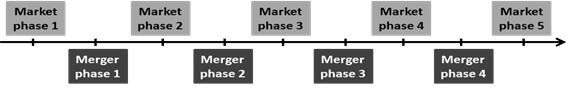
\includegraphics[width=0.8\linewidth]{phases} \\
	\end{centering}
	\footnotesize Note: Merger to monopoly not possible. In addtion, only one merger phase allowed. 
\end{figure}

\newpage

% Heatmap


\newpage

\begin{figure}
    \begin{center}
        \includegraphics[width=0.8\linewidth]{plot.pgf}
    \end{center}
    \caption{Plot with 4 lines, colorblind-friendly}
\end{figure}

\newpage


\section{Discussion}

\blindtext

\newpage







\section{References}
\begingroup
\renewcommand{\section}[2]{}
\nocite{*}
\printbibliography
\endgroup

\newpage




\end{document}
